\documentclass[12pt,a4paper,handout]{beamer}

\usefonttheme{professionalfonts}
%\usepackage[ngerman]{babel}% deutsches Sprachpaket wird geladen
\usepackage[ngerman,english]{babel}% englisches Sprachpaket wird geladen
\usepackage{tabularx}
\usepackage{lmodern}% Für die Schrift
\usepackage[T1]{fontenc} % westeuropäische Codierung wird verlangt
\usepackage[utf8]{inputenc}% Umlaute werden erlaubt
\usetheme{Berlin}
    \expandafter\def\expandafter\insertshorttitle\expandafter{%
    \insertshorttitle\hfill%
    \insertframenumber\,/\,\inserttotalframenumber}
%\usepackage{showkeys} % Labels anzeigen
\usepackage{amsmath} % Erweiterung für den Mathe-Satz
\usepackage{amssymb} % alle Zeichen aus msam und msmb werden dargestellt
\usepackage{framed}
\usepackage[german]{fancyref}
\usepackage{listings}
\usepackage{color}
\definecolor{mygreen}{RGB}{28,172,0} % Define colour
\definecolor{mylilas}{RGB}{170,55,241}
\usepackage{graphicx} % Graphiken und Bilder können eingebunden werden
\usepackage{multirow} % erlaubt in einer Spalte einer Tabelle die Felder in mehreren Zeilen zusammenzufassen
\usepackage{url} % Dient zur Auszeichnung von URLs; setzt die Adresse in Schreibmaschinenschrift.
\usepackage[center]{caption}  % Bildunterschrift wird zentriert
\usepackage{subfigure} % mehrere Bilder können in einer figure-Umgebung verwendet werden
\usepackage{longtable} % Diese Umgebung ist ähnlich definiert wie die tabular-Umgebung, erlaubt jedoch mehrseitige Tabellen.
\usepackage{amsthm} % erlaubt die Benutzung von eigenen Theoremen
\usepackage{hyperref} % Links und Verweise werden innerhalb von PDF Dokumenten erzeugt
\usepackage{wrapfig} % Das Paket ermöglicht es von Schrift umflossene Bilder und Tabellen einzufügen.
%\numberwithin{equation}{section} % Nummerierungen der Gleichungen, die durch equation erstellt werden, sind gebunden an die section
\usepackage{latexsym} % LaTeX-Symbole werden geladen
\usepackage{tikz} % Erlaubt es mit tikz zu zeichnen
\usepackage{tabularx} % Erlaubt Tabellen 
\usepackage{algorithm} % Erlaubt Pseudocode
\usepackage{algorithmic}
\usepackage{color} % Farbpaket wird geladen
\usepackage{stmaryrd} % St Mary Road Symbole werden geladen
\usepackage{csquotes}
\usepackage{bm}
\usepackage{todonotes}
\usepackage{lipsum}
\usepackage{multicol}
\usepackage{multimedia}

% Hier werden neue Theorems erstellt.
\theoremstyle{definition}
\newtheorem{auf}{Aufgabe}
\newtheorem{rem}[auf]{Remark}
\newtheorem{defn}[auf]{Definition}
\newtheorem{bsp}[auf]{Example}
\newtheorem{notation}[auf]{Notation}
\theoremstyle{plain}
\newtheorem{kor}[auf]{Corollary}
\newtheorem{sa}[auf]{Theorem}
\newtheorem{lem}[auf]{Lemma}
\newtheorem{alg}[auf]{Algorithm}
\DeclareMathOperator*{\esssup}{ess\,sup} % essentiellen Supremums
\DeclareMathOperator{\spn}{span} % Span
\DeclareMathOperator{\supp}{supp} % Träger
\DeclareMathOperator{\ddiv}{div} % divergenz
\newcommand{\abs}[1]{\left\vert #1\right\vert}
\newcommand{\dotp}[2]{\left\langle #1,#2\right\rangle}
\newcommand{\rr}{\mathbb{R}}
\newcommand{\g}{~\textgreater ~}
\newcommand{\ls}{~\textless ~}
\renewcommand{\algorithmicrequire}{\textbf{Input:}}
\renewcommand{\algorithmicensure}{\textbf{Output:}}
\newcommand{\cc}{\mathbb{C}}
\newcommand{\kk}{\mathbb{K}}
\newcommand{\nn}{\mathbb{N}}
\newcommand{\qq}{\mathbb{Q}}
\newcommand{\e}{\varepsilon\g 0~}
\newcommand{\fe}{\forall \e}
\newcommand{\so}{\sum_{k=0}^{n}}
\newcommand{\si}{\sum_{k=1}^{n}}
\newcommand{\soi}{\sum_{k=0}^{\infty}}
\newcommand{\sii}{\sum_{k=1}^{\infty}}
\newcommand{\de}{\mathrm{d}}
\newcommand{\norm}[1]{\left\lVert#1\right\rVert}
\newcommand{\lpnorm}[1]{\left(\int\abs{#1}^2\D\Omega \right)^{1/2}}
\newcommand{\bfu}{\bm{u}}
\newcommand{\bff}{\bm{f}}
\newcommand{\bfB}{\bm{B}}
\newcommand{\bfb}{\bm{b}}
\newcommand{\bfs}{\bm{s}}
\newcommand{\bfC}{\bm{C}}
\newcommand{\bfx}{\bm{x}}
\newcommand{\bfR}{\bm{R}}
\newcommand{\D}{\mathop{}\!\mathrm{d}}
\floatname{algorithm}{Algorithmus}
%\renewcommand{\thesubfigure}{the.g}
\addto{\captionsenglish}{\renewcommand{\bibname}{References}}
\lstset{language=Matlab,
    basicstyle={\scriptsize \ttfamily},
    breaklines=true,
    morekeywords={matlab2tikz},
    keywordstyle=\color{blue},
    morekeywords=[2]{1}, 
    keywordstyle=[2]{\color{black}},
    identifierstyle=\color{black},
    stringstyle=\color{mylilas},
    commentstyle=\color{mygreen},
    showstringspaces=false, %without this there will be a symbol in the places where there is a space
    numbers=left,
    numberstyle={\tiny \color{black}}, % size of the numbers
    numbersep=9pt, % this defines how far the numbers are from the text
    emph=[1]{for,end,break},
    emphstyle=[1]\color{red}, %some words to emphasise
}
\makeatletter
\renewcommand{\p@subfigure}{}
\renewcommand{\@thesubfigure}{\thesubfigure:\hskip\subfiglabelskip}
\makeatother
\begin{document}
    \title{Numerical Solution of Integro-Differential Equations}
    \author{Nils Dornbusch}
    \date{September 26, 2019}
    \maketitle
   
\section{Motivation}
\begin{frame}
    \frametitle{Motivation}
    For a \textsc{Newtonian} fluid it holds that
    \begin{equation*}
        \text{shear stress} \propto \text{strain.}
    \end{equation*}
    However, for many fluids this relationship is not valid. We call them non-\textsc{Newtonian} fluids.
\end{frame}
\begin{frame}
     \frametitle{Introduction}
    There are many examples for non-\textsc{Newtonian} fluids. These include
    \begin{itemize}[<+->]
        \item toothpaste
        \item liquid plastic
        \item granular flow
        \item and many more.
    \end{itemize}
\end{frame}

\begin{frame}
\frametitle{The incompressible Navier Stokes equations}
    \begin{align*}
        \frac{\partial \bfu}{\partial t}+(\bfu\cdot \nabla)\bfu &= \bff +\nabla\cdot\sigma +\mu_s\Delta\bfu-\nabla p,\\
        \ddiv(\bfu)&= 0,\\
        \sigma(t,\hat\bfx)&= \int_{-\infty}^t-\partial_{t'}\bfB(t,t',\hat\bfx)G(t,t')\D t',\\
        \partial_t \bfB &=- (\bfu\cdot\nabla)\bfB+(\nabla \bfu)\bfB+\bfB(\nabla\bfu)^T.
    \end{align*}
with e.g. $G(t,t')=\mu_p\cdot e^{-(t-t')/\lambda}$, $\bfu$ the velocity vector, $\bff$ a generic source term, $\sigma$ the stress tensor, $\mu_s, \mu_p$ the solvent and polymer viscosity respectively, $p$ the pressure, $\lambda$ the relaxation time and $\bfB$ the Finger tensor.
\end{frame}
 \begin{frame}
     \frametitle{Boundary conditions}
     We choose suitable initial and boundary conditions for the velocity. For $\bfB$ we use
     \begin{align*}
         \bfB(t,t,\hat\bfx)& = \bm{1},\\
         \bfB(0,t',\hat\bfx) &=\bm{1},
     \end{align*}
     which means that we assume a stress free start of the simulation.
 \end{frame}
\begin{frame}
\frametitle{Another possibility for $G$}
In more advanced physical models, $G$ is given by $G\propto\phi^2$, where $\phi$ is defined as the solution of 
\begin{align*}
\dot\phi(t)&=-\phi(t)-\int_0^tm(t-\tau)\dot\phi(\tau)\D\tau,\\
m(t)&=v_1\phi(t)+v_2\phi(t)^2,
\end{align*}
where we choose $v_1,v_2\in\rr$.
\end{frame}
\begin{frame}
\frametitle{Motivation}
\begin{itemize}[<+->]
    \item Physical interest in e.g. a glass transition of a fluid or granular flow
    \item Simulation of this particular fluid model does not exist 
    \item First step in trying to develop a stable numerical approach
    \item To develop a starting point for future projects
\end{itemize}
\end{frame}
\begin{frame}
    \frametitle{Outline}
    The talk will have two main parts:
    \begin{itemize}
        \item \textsc{Navier-Stokes} equations for $G=\sum_{i=1}^{n}\mu_p^{(i)}e^{-(t-t')/\lambda_i}$
        \item Look at the equation for $\phi$ only to study different approaches
    \end{itemize}
\end{frame}
\begin{frame}
    \Huge{Part I: \textsc{Navier-Stokes} equations}
\end{frame}
\section{3D to 2D reduction}
    \begin{frame}
        \frametitle{Assumptions for the dimension reduction}
        These are very complex equations. This work uses the following assumptions:
        \begin{itemize}[<+->]
            \item $\bfu= (0,0,u)^T$, $\bff=\bm{0}$, $\nabla p\equiv(0,0,\partial_3 p)$
            \item $\partial_3\bfB =\bm{0}$
         \end{itemize}
    \uncover<3->{This yields a 2D model for the cross sectional flow in a e.g. tube.}\\
    
    \only<4>{\begin{figure}
            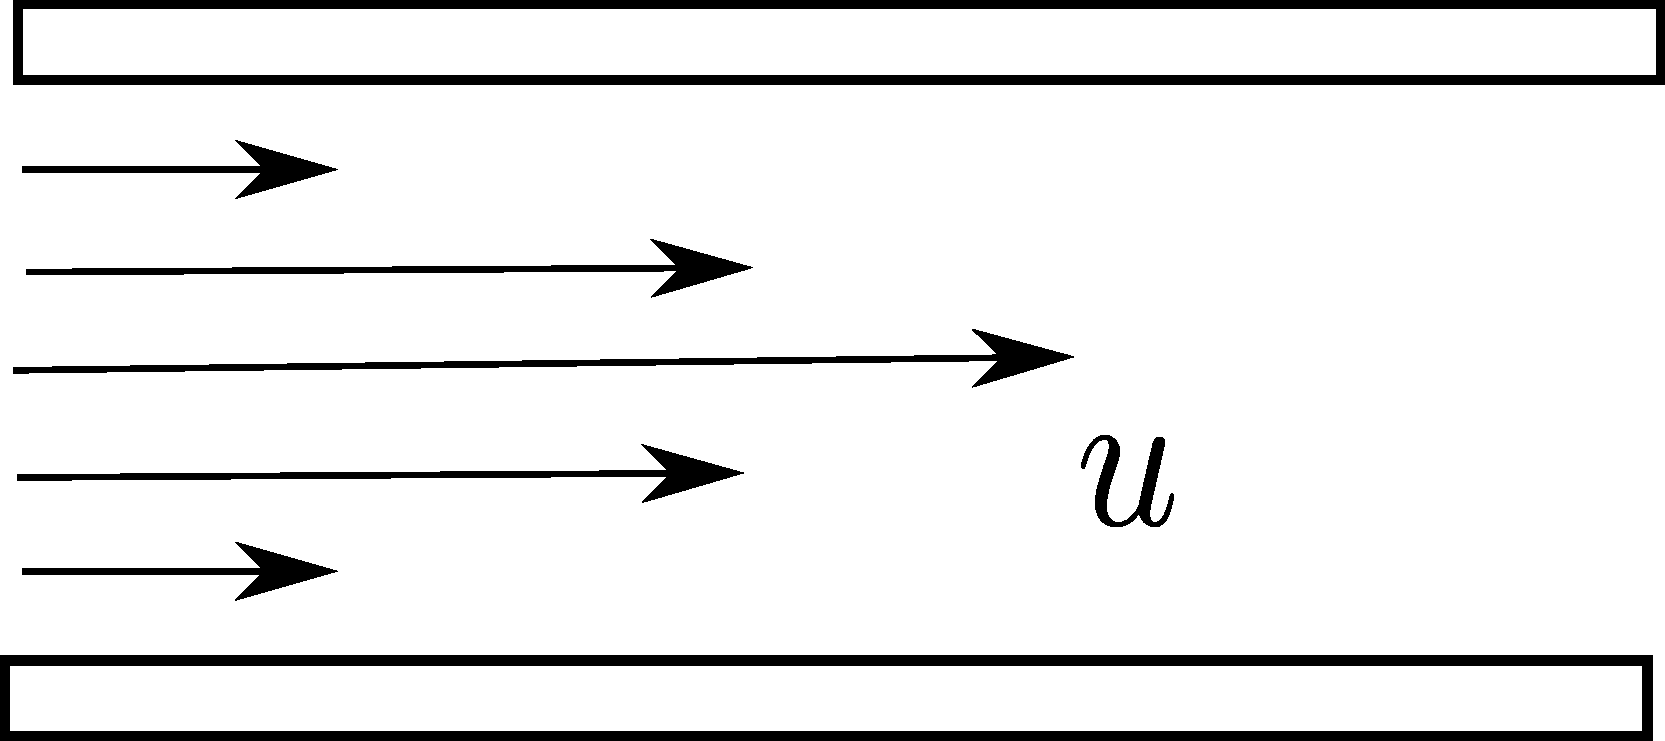
\includegraphics[width=0.5\textwidth]{laminarflow}
            \caption{Visualization of the assumptions}
         \end{figure}}
    \end{frame}
\begin{frame}
    \frametitle{Introducing new variables}
    We define
     \begin{equation*}
    \bfB=\begin{pmatrix}
    1&0&\bfb_1\\
    0&1&\bfb_2\\
    \bfb_1&\bfb_2&*
    \end{pmatrix}
    \end{equation*}
    and
    \begin{equation*}
        s:=\sigma_{3,j},\quad \text{for }j=1,2
    \end{equation*}
\end{frame}
\begin{frame}
    \frametitle{Reduced 2D equations}
    These assumptions yield the 2D equations 
    \begin{align*}
    \partial_t u(t,\bfx) &= -\partial_3 p +\nabla\cdot \bfs+\mu_s\Delta u,\\
    \bfs(t,\bfx) &=\int_{-\infty}^t-\mu_p\partial_{t'}\bfb(t,t',\bfx)e^{-(t-t')/\lambda}\D t',\label{eq:s2D}\\
    \partial_t\bfb(t,t',\bfx)&=
    \begin{pmatrix}
    \partial_1 u(t,\bfx)\\\partial_2 u(t,\bfx)
    \end{pmatrix}=\nabla u.
    \end{align*}
\end{frame}
\begin{frame}
    \frametitle{\textsc{Laplace} transform}
    We want to eliminate \begin{equation*}
        \bfs(t,\bfx)=\int_{-\infty}^t-\mu_p\partial_{t'}\bfb(t,t',\bfx)e^{-(t-t')/\lambda}\D t'
    \end{equation*}
    To achieve this, introduce $\tau=t-t'$ (age variable) to obtain
    \begin{equation*}
    \bfs(t,\bfx)=\int_0^\infty\mu_p\partial_\tau\bfb(t,t-\tau,\bfx)e^{-(t-t')/\lambda}\D\tau.
    \end{equation*}
    Using the chain rule the governing equation for the \textsc{Finger} tensor transforms to  
    \begin{equation*}
    \partial_t \bfb +\partial_\tau\bfb=\nabla u.
    \end{equation*}
\end{frame}
\begin{frame}
    \frametitle{\textsc{Laplace} transform}
    Use $\bfb\mapsto \mathcal{L}_\tau\{\bfb\}:=\int_0^\infty \bfb(x,t,t-\tau)e^{-s\tau}\D \tau$ to transform
    \begin{equation*}
    \partial_t \bfb +\partial_\tau\bfb=\nabla u.
    \end{equation*}
     This yields
    \begin{equation*}
    \partial_t\mathcal{L}_\tau\{\bfb\}(t,\bfx,s) + \mathcal{L}_\tau\{\partial_\tau\bfb\}(t,\bfx,s) = \frac{1}{s}\nabla u.
    \end{equation*} Using the transformation rules for the \textsc{Laplace} transform results in
    \begin{equation*}
        (\partial_t +s)\mathcal{L}_\tau{\bfb}(t,\bfx,s) = \frac{1}{s}\nabla u.
    \end{equation*}
\end{frame}
\begin{frame}
    \frametitle{\textsc{Laplace} transform}
    Using the conformation tensor $\bfC_s:=s\mathcal{L}_\tau{\bfb}(t,\bfx,s)$ we obtain
    \begin{equation*}
         \partial_t\bfC_s(t,\bfx)+s\bfC_s(t,\bfx)=\nabla u.
    \end{equation*}
    If we set $s:=\frac{1}{\lambda}$, it follows
    \begin{equation*}
        \bfs(t,\bfx)=\mu_p\bfC_{1/\lambda}(t,\bfx).
    \end{equation*}
\end{frame}
\begin{frame}
    \frametitle{The transformed 2D equations}
    \begin{align*}
        \partial_t u(t,\bfx) &= -\partial_3 p +\nabla\cdot \bfs+\mu_s\Delta u,\\
        \label{eq:transfeq2}
        \bfs(t,\bfx)&=\mu_p\bfC_{1/\lambda},\\
        \partial_t\bfC_{1/\lambda}(t,\bfx) &= -\frac{1}{\lambda}\bfC_{1/\lambda}(t,\bfx)+\nabla u    \end{align*}
        This is a linear system of which the existence and uniqueness of the solution is proven in the thesis for $\mu_s>0$ in the weak formulation.
\end{frame}
\section{Numerics}
\begin{frame}[fragile]
    \frametitle{The software}
    The software used is FEniCS. 
    \begin{itemize}[<+->]
        \item Framework for solving PDEs with finite element discretization (limited DG support available)
        \item have to plug in the weak form and maybe time loop
    \end{itemize}
A Code example:
\begin{verbatim}
F = u * v * dx - un3 * v * dx + dt * (gradP * v * dx 
  + dot(mup * as_vector([C1, C2]), grad(v)) * dx 
  + mus * dot(grad(u), grad(v)) * dx) 
  + (C1 - un1 + dt / Lambda * C1) * CV1 * dx 
  + (C2 - un2 + dt / Lambda * C2) * CV2 * dx 
  - dt * dot(grad(u), as_vector([CV1, CV2])) * dx
\end{verbatim}
\end{frame}
\begin{frame}
    \frametitle{Setup startup flow}
    
    \begin{figure}
        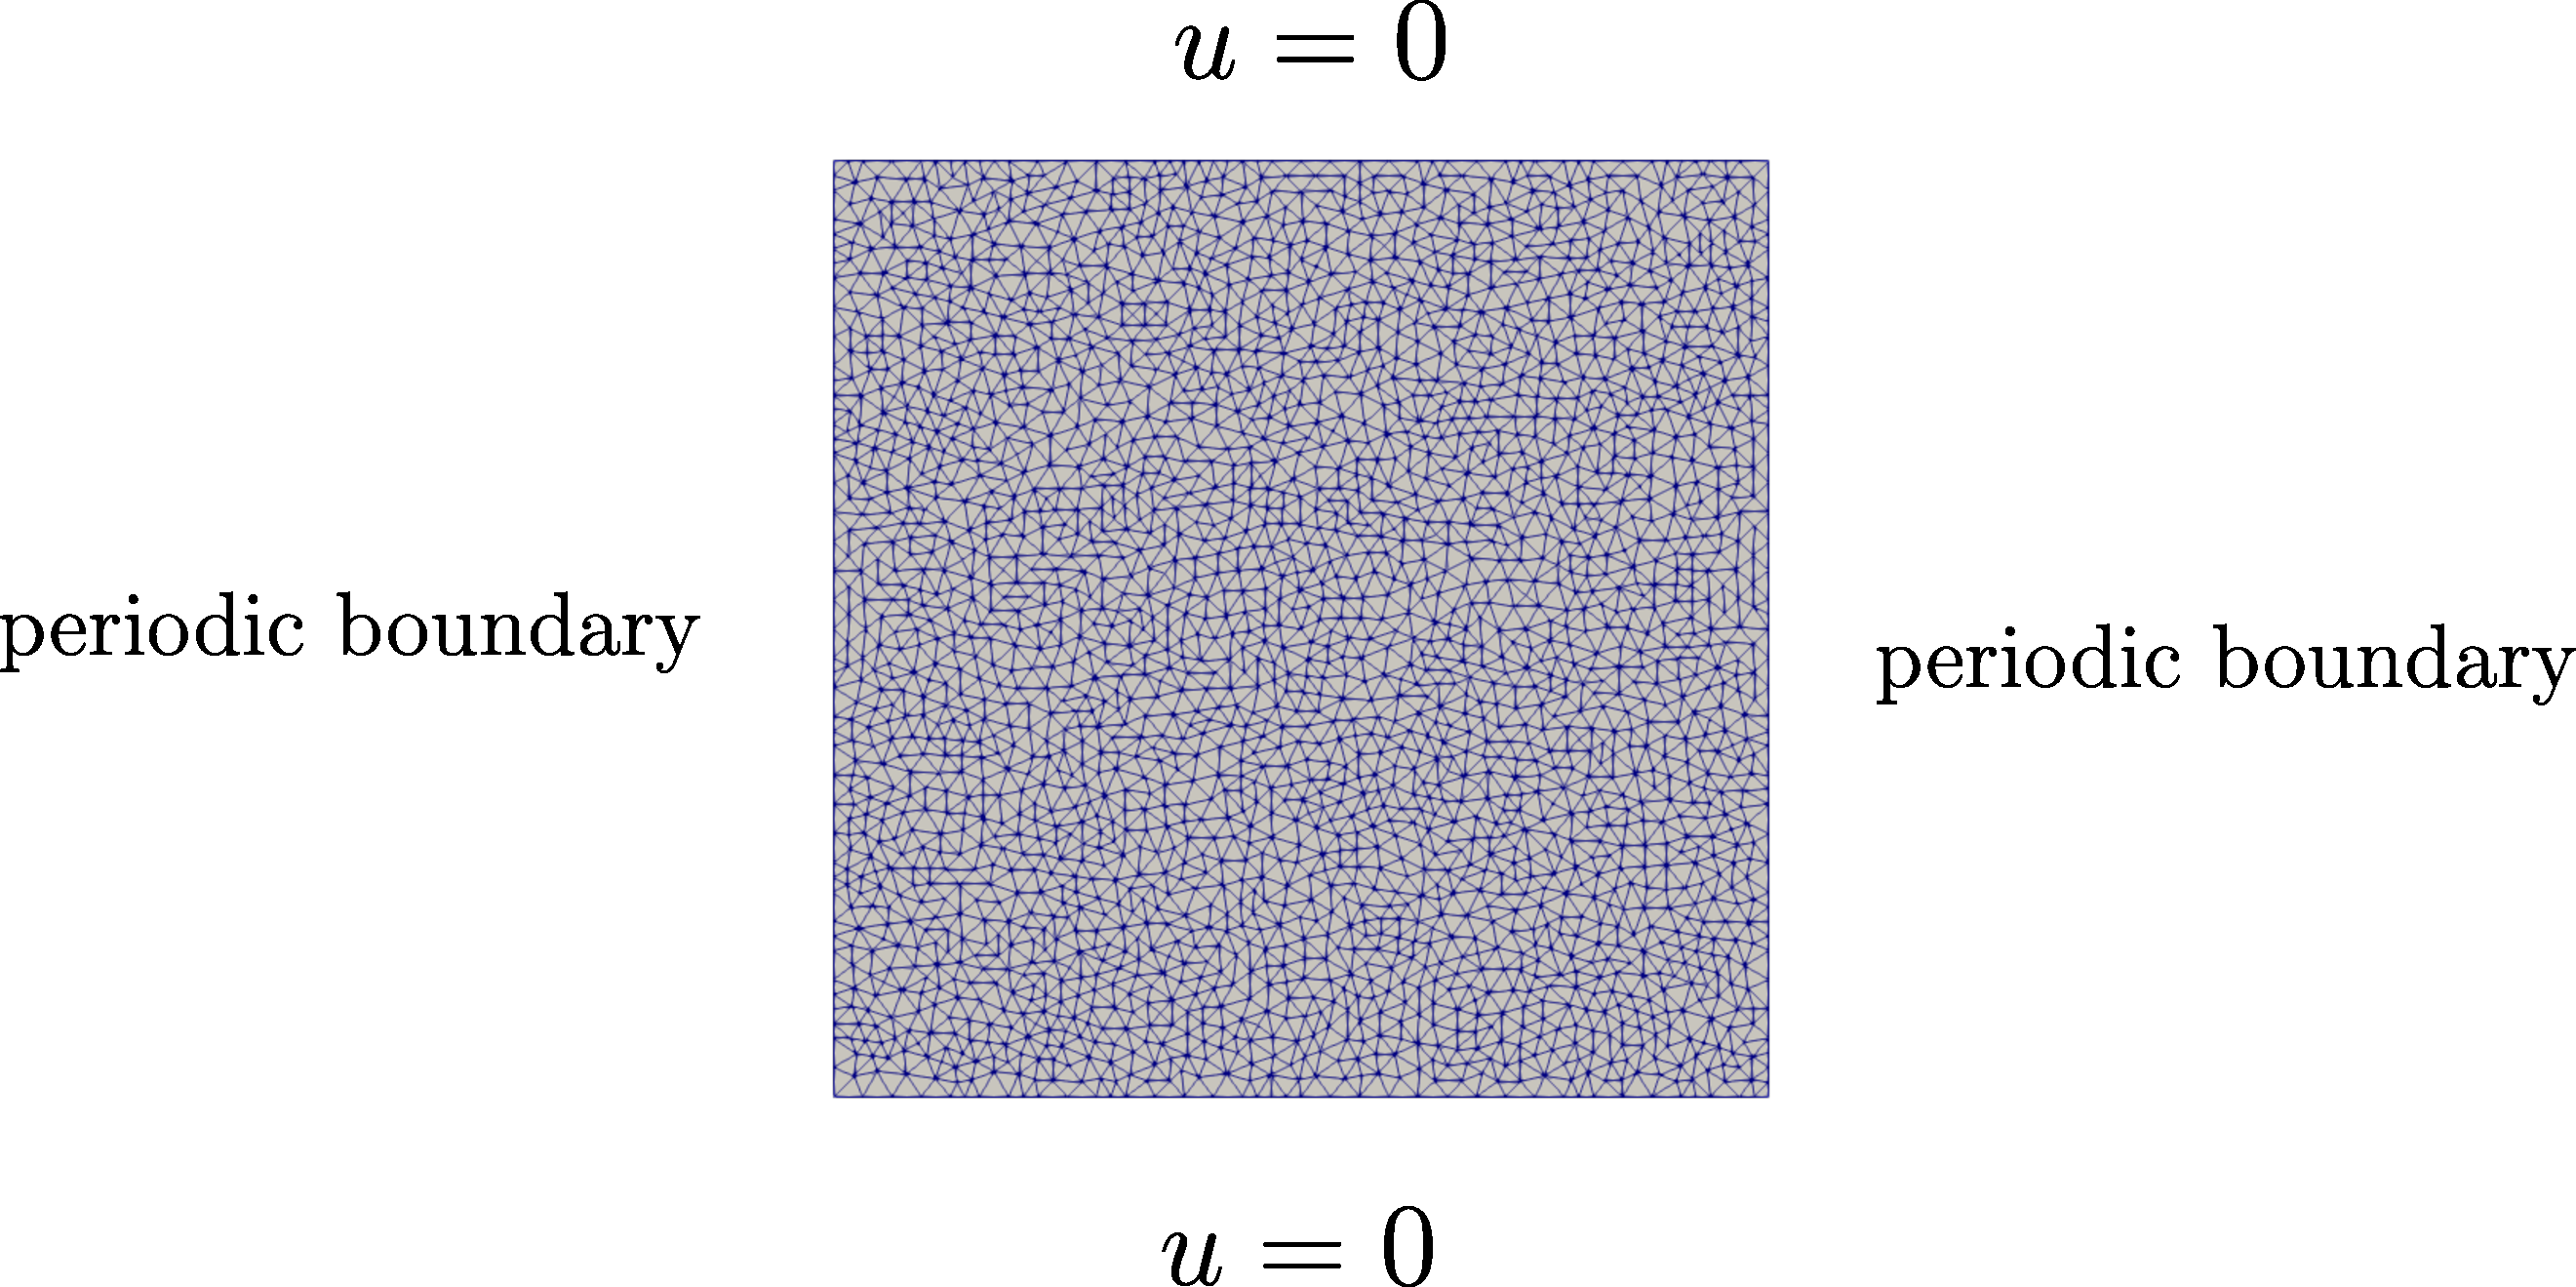
\includegraphics[width=0.8\textwidth]{setupsquare}
    \end{figure}
\end{frame}

\begin{frame}
    \frametitle{Startup flow}
    \begin{figure}
        \centering
        \subfigure{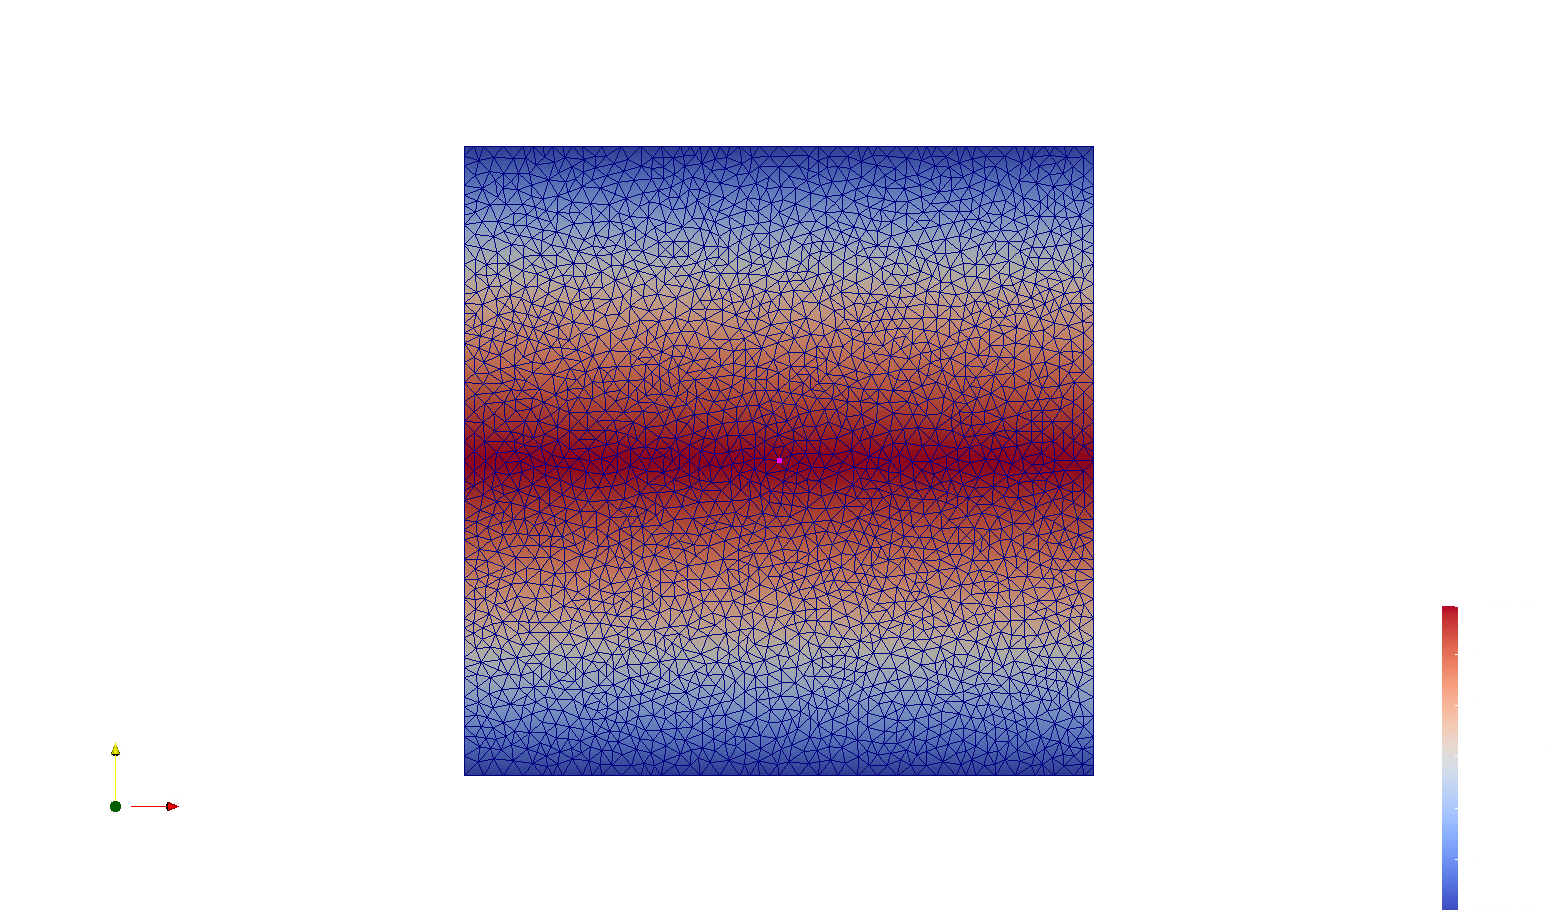
\includegraphics[width=0.4\textwidth]{vel}}
        \subfigure{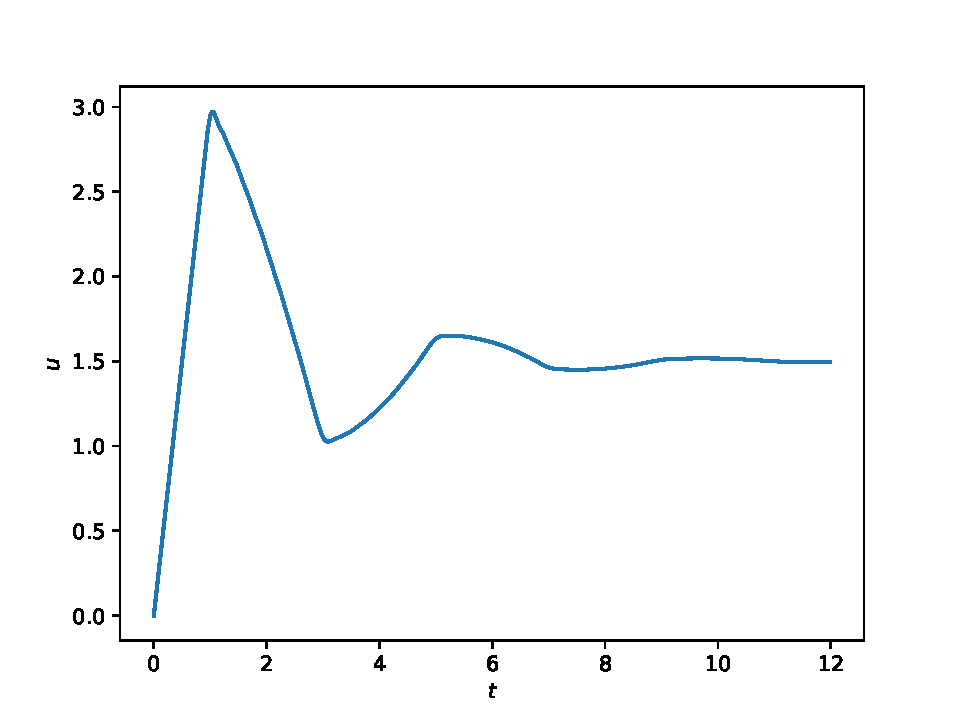
\includegraphics[width=0.55\textwidth]{centerlinevel.pdf}}
        \caption{Startup flow Maxwell with $\lambda=1,\mu_p=1$ and $\partial_3p=-3$}
    \end{figure}
\end{frame}
\begin{frame}
    \frametitle{Numerical results}
    Convergence in the $L^2$-norm was achieved with a timestep width of $0.1$ and an end time of $1$ for a manufactured solution on a unit disc.
    \begin{table}
        \centering
        \begin{tabular}{c|c|c}
            $\approx$ \# Elements per diameter& $\mathrm{L}^2$-error&EOC\\
            \hline
            20 & 0.0797652 & -\\
            40 & 0.0233543 & 1.77207\\
            80 & 0.00615334 & 1.92425\\
            160 & 0.00163421 & 1.91278\\
            320 & 0.000433982 & 1.91288
        \end{tabular}
        \caption{Convergence of the \textsc{Maxwell} model $(\mu_s=0)$}
    \end{table}
\end{frame}
\begin{frame}
    \frametitle{Setup rheometer}
    We choose $\lambda =2,\,\mu_p=0.9,\,\mu_s=0.1$ and $\partial_3 p=0$.
    \begin{figure}
        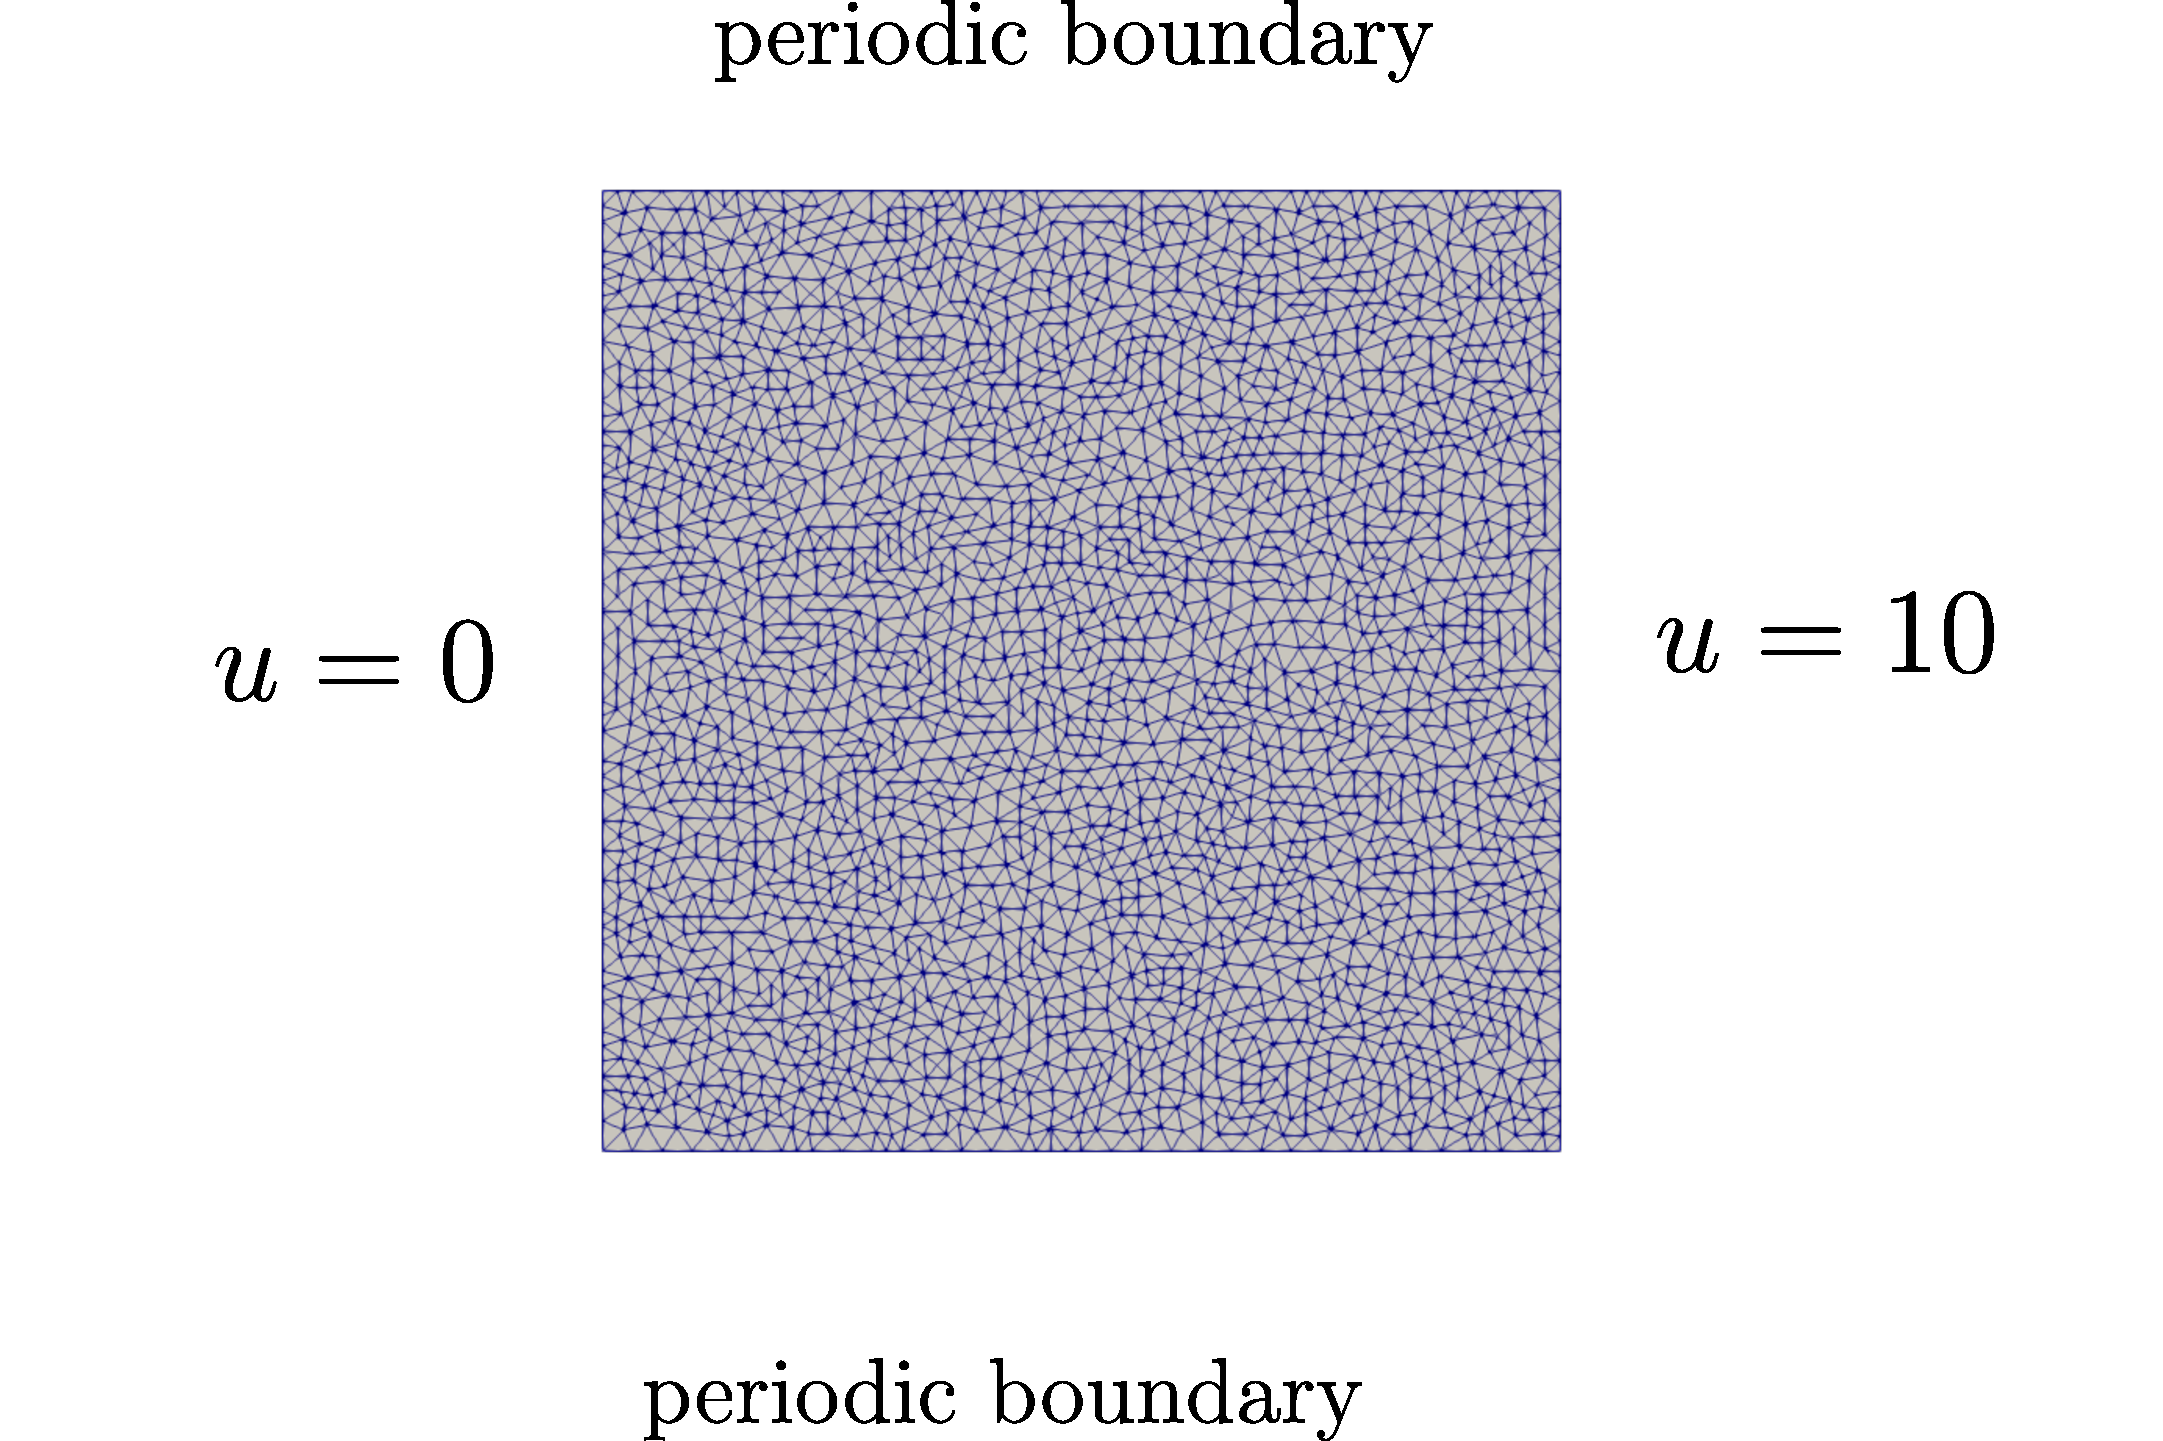
\includegraphics[width=0.8\textwidth]{setuprheo}
    \end{figure}
\end{frame}
\begin{frame}
    \frametitle{Cross section of an ideal rheometer}
    
\end{frame}
\section{Other approaches for the integral eq.}
\begin{frame}
\frametitle{Different approaches for the integral equation}
    What happens if the \enquote{\textsc{Laplace} trick} is not possible? 
    \begin{itemize}[<+->]
        \item look at a combination of multiple relaxation times
        \item brute force (mainly as reference)
        \item exponentially increasing time intervals
        \item transformation of the argument
    \end{itemize}
\end{frame}
\begin{frame}
    \frametitle{Combination of relaxation times}
    Let $(\lambda_i)_{i=1,\dotsc,N},(\mu_p^i)_{i=1,\dotsc,N}$ be a sequence of relaxation times and polymer viscosities respectively. We set
    \begin{equation*}
    G(\tau)=\sum_{n=1}^{N}\mu_p^{(n)}e^{-\tau/\lambda_n},
    \end{equation*}
\end{frame}
\begin{frame}
    \frametitle{Combination of relaxation times}
    Putting $G$ into the governing equation yields
    \begin{equation*}
    \bfs(t) = \sum_{n=1}^{N}\mu_p^{(n)}\int_0^t\partial_\tau \bfb(t,t-\tau)e^{-\tau/\lambda_n}\D\tau.
    \end{equation*}
    Using similar arguments as before results in 
    \begin{equation}
    \bfs(t)=\sum_{n=1}^N\frac{\mu_p^{(n)}}{\lambda_n}L_{\bfb}(t,1/\lambda_n)=\sum_{n=1}^N\mu_p^{(n)}\bfC_{1/\lambda_n}.
    \end{equation}
\end{frame}
\begin{frame}
    \frametitle{Combination of relaxation times}
    \begin{figure}
        \centering
        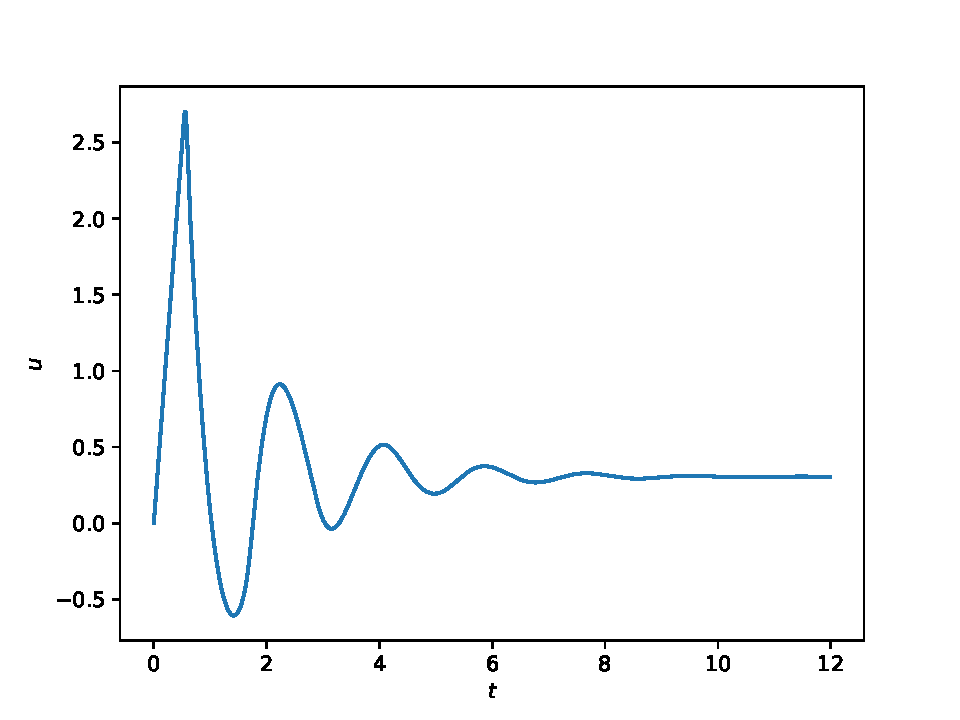
\includegraphics[width=0.5\textwidth]{multilam}
        \caption{startup flow with $\lambda=\{0.1,1,3\}$ and $\mu_p=1$}
    \end{figure}
\end{frame}
\begin{frame}
\frametitle{Combination of relaxation times}
    How do we interpret the result?
    \begin{itemize}[<+->]
        \item qualitatively behavior of non-\textsc{Newtonian} fluid
        \item similar to previous results
        \item extrema seem to be at multiples of the geometric mean ($\approx 0.66$)  
    \end{itemize}
\end{frame}
\begin{frame}
    \frametitle{Combination of relaxation times}
    Advantages and disadvantages
    \begin{itemize}[<+->]
        \item For each relaxation time we obtain
        \begin{equation*}
            \partial_t \bfC_{1/\lambda_n}+\frac{1}{\lambda_n}\bfC_{1/\lambda_n}=\nabla u
        \end{equation*}
        \item more equations $\Rightarrow$ more computational effort
        \item we retain existence and uniqueness of solution
    \end{itemize}
\end{frame}
\begin{frame}
    \frametitle{Introducing a new equation}
    Remaining two approaches considered on
    \begin{align*}
    \dot\phi(t)&=-\phi(t)-\int_0^tm(t-\tau)\dot\phi(\tau)\D\tau,\\
    m(t)&=v_1\phi(t)+v_2\phi(t)^2,
    \end{align*}
    with $v_1,v_2\in\rr$ parameters. Why do we use these instead?
    \begin{itemize}[<+->]
        \item fewer dimensions and equations
        \item same difficulty regarding the integral
        \item easier to test methods
    \end{itemize}
\end{frame}
\begin{frame}
    \frametitle{Introducing a new equation}
    We can transform the previous equation to 
    \begin{equation*}
        \phi(t)=\phi(0)+\int_0^t[m(\tau)(\phi(0)-\phi(t-\tau))-\phi(\tau)]\D \tau.
    \end{equation*}
    We discretize $t$ with $0=t_0,\dotsc,t_N=T$, where $T$ is the end time.
\end{frame}
\begin{frame}
    \frametitle{Brute force algorithm}
    By using equal distant points $t_j$ and the trapezoidal rule we obtain the brute force algorithm. Drawbacks:
    \begin{itemize}[<+->]
        \item computational effort $\mathcal{O}(N^2)$
        \item the calculation of each time step $t_{n+1}$ is more expensive than $t_{n}$ for all $n$
    \end{itemize}
    We use it to verify the other ideas.
\end{frame}
\begin{frame}
    \frametitle{Exponentially increasing time intervals}
    Idea behind this approach:
    \begin{itemize}[<+->]
        \item $\phi$ is exponentially declining in $t$
        \item similar trick used in Fast-\textsc{Fourier}-Transformation
    \end{itemize}
We set $t_j=h2^j$ for $j=1,\dotsc N$ and use the quadrature rule
\begin{equation*}
    \int_0^{t_n}f(t)dt=\sum_{j=0}^{n-1}\int_{t_j}^{t_{j+1}}f(t)\D t\approx\sum_{j=0}^{n-1}(t_{j+1}-t_j)f_{j+1}
\end{equation*}
for a generic function $f$.
\end{frame}
\begin{frame}
    \frametitle{Exponentially increasing time intervals}
    Using the quadrature rule yields
    \begin{equation*}
        \phi_n = \phi_0 + \sum_{j=0}^{n-1}h_j[m_{j+1}(\phi_0-\phi(t_n-t_{j+1}))-\phi_{j+1}].
    \end{equation*}
    The update from $\phi_n$ to $\phi_{n+1}$ is given by
    \begin{equation*}
        \phi_{n+1}= \phi_n -h_n\phi_{n+1}+\sum_{j=0}^{n-1}h_jm_{j+1}(\phi(t_n-t_{j+1})-\phi(t_{n+1}-t_{j+1})).
    \end{equation*}
\end{frame}
\begin{frame}
    \frametitle{Exponentially increasing time intervals}
    We have the problem that $t_n-t_{j+1}$ and $t_{n+1}-t_{j+1}$ are not equal to $t_j$ for some $j$ in general. The solution is interpolating $t_n-t_{j+1}\approx t_n$ and $t_{n+1}-t_{j+1}\approx t_{n+1}$. After reordering we obtain
    \begin{equation*}
         \phi_{n+1}(1 + h_n + \sum_{j=0}^{n-2}h_jm_{j+1})=\phi_n(1+\sum_{j=0}^{n-2}h_jm_{j+1})+h_{n-1}m_n(\phi_0-\phi_n).
    \end{equation*}
\end{frame}
\begin{frame}
    \frametitle{Exponentially increasing time intervals}
    Now we have to take care of the sums. We multiply both sides by $2^{-n}$ and set $\beta_n=2^{-n}\sum_{j=0}^{n-2}h_jm_{j+1}$. It yields
    \begin{align*}
    \phi_{n+1}(2^{-n}+h+\beta_n) &= \phi_n(2^{-n}+\beta-\frac{h}{2}m_n)+\frac{h}{2}m_n\phi_0,\\
    \beta_{n+1} &= \frac{1}{2}(\beta_n+\frac{h}{2}m_n).
    \end{align*}
\end{frame}
\begin{frame}
    \frametitle{Analysis of exp. increasing time intervals}
    How do we interpret the results?
    \begin{itemize}[<+->]
        \item computational effort $\mathcal{O}(N)$
        \item unclear if $h\to 0$ converges to the solution
        \item error to great (interpolation to bad?)
        \begin{figure}
            \centering
            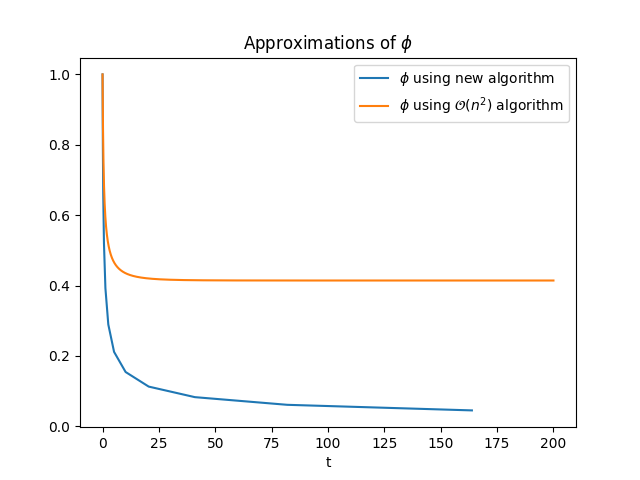
\includegraphics[width=0.4\textwidth]{Phidiff}
            \caption{Both $\phi$ with $h=\Delta t=0.01$ and $v_1=1.5,~v_2=0.5$}
        \end{figure}
    \end{itemize}
\end{frame}
\begin{frame}
    \frametitle{Transformation of the argument}
    Idea for this approach:
    \begin{itemize}
        \item transform $t=f(u)$ to obtain better properties for the integral
    \end{itemize}
    Inserting this transformation and setting $\tilde\phi(u)=\phi(f(u))$ yields
    \begin{align*}
        \tilde{\phi}(u)&=\tilde{\phi}(u_{-1}) +\int_{u_{-1}}^{u}f'(u')[\tilde{m}(u')(\tilde\phi(u_{-1})\\&-\tilde{\phi}(f^{-1}(f(u)-f(u'))))-\tilde{\phi}(u')]\D u',
    \end{align*}
    where $u_{-1}=f^{-1}(0)$.
\end{frame}
\begin{frame}
    \frametitle{Transformation of the argument}
    The problematic part is
    \begin{equation*}
        \int_{u_{-1}}^{u}f'(u')\tilde{m}(u')\tilde{\phi}(f^{-1}(f(u)-f(u')))\D u'.
    \end{equation*}
    Ideally,
    \begin{equation*}
        F(u,u'):=f^{-1}(f(u)-f(u'))=u
    \end{equation*}
    almost everywhere.
\end{frame}
\begin{frame}
    \frametitle{Transformation of the argument}
    \begin{figure}
        \centering
        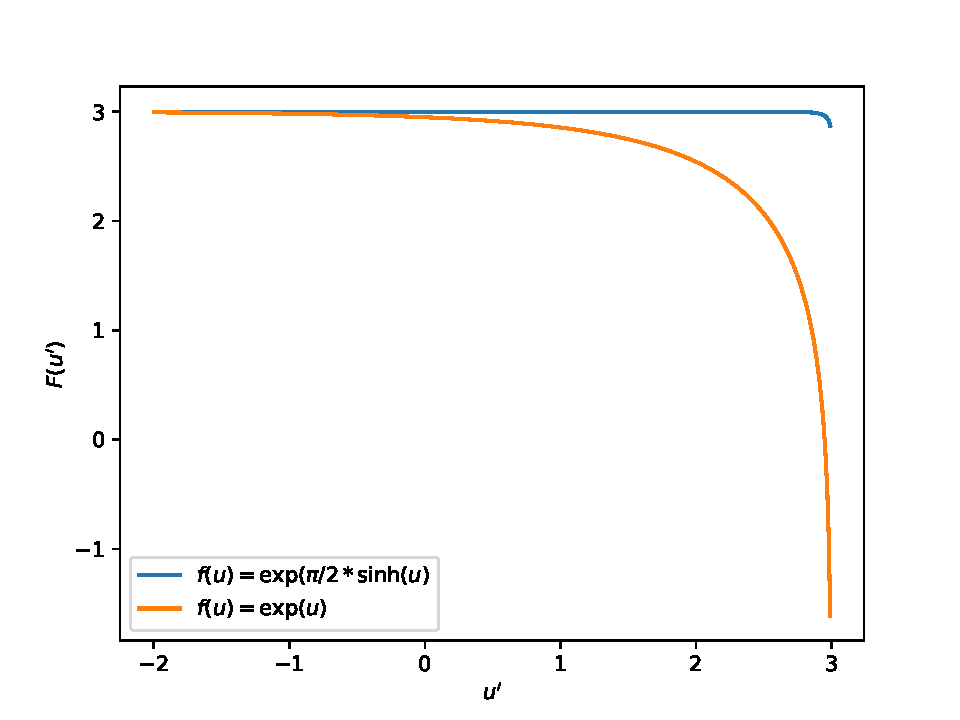
\includegraphics[width=0.8\textwidth]{HistoryF}
        \caption{History dependency for different $f$}
    \end{figure}
\end{frame}
\begin{frame}
    \frametitle{Transformation of the argument}
    Interpretation of this figure:
    \begin{itemize}[<+->]
        \item Both have a sharp drop in the end
        \item $f(u)=\exp(\pi/2\sinh(u))$ is better suited in this regard
        \item but it results in a qualitatively different curve for each $u$
        \item we take $f(u)=\exp(u)$ because of this 
    \end{itemize}
\end{frame}
\begin{frame}
    \frametitle{Transformation of the argument}
    We only discuss $\int_{u_{-1}}^{u}f'(u')\tilde{m}(u')\tilde{\phi}(f^{-1}(f(u)-f(u')))\D u'$ here. We use $u_j=u_0+jh$ with $j=0,\dotsc,N$ and $\abs{f(u_0)-f(u_{-1})}$ sufficiently small. We obtain
    \begin{equation*}
        I_2:=\int_{u_{-1}}^{u_{n+1}}f'(v)\tilde{m}(v)\tilde{\phi}(F(u_{n+1},v))\D v
    \end{equation*}
\end{frame}
\begin{frame}
    \frametitle{Transformation of the argument}
    The big question is: Which integration points do we use for $I_2$? Observe that
    \begin{equation*}
        w=F(u,u')\Rightarrow u'=F(u,w).
    \end{equation*}
    We define 
    \begin{equation*}
        w_{i}^{n}:=F(u_n,u_i).
    \end{equation*}
    Then we use the discretization 
    \begin{equation*}
        (v_i)_{i=0,\dotsc,2n+1}=\text{sorted}\{(u_i)_{i=0,\dotsc,n}\cup (w^n_{i})_{i=0,\dotsc,n-1}\}
    \end{equation*}
\end{frame}
\begin{frame}
    \frametitle{Transformation of the argument}
    This is possible because we assume
    \begin{equation*}
        \tilde\phi(v)=\tilde{\phi}(u_i)\quad\forall v\in (u_{i-1},u_i]
    \end{equation*}
    for all $i=0,\dotsc,N$ so we use constant ansatz functions on each interval.
\end{frame}
\begin{frame}
\frametitle{Transformation of the argument}
    \begin{figure}
        \centering
        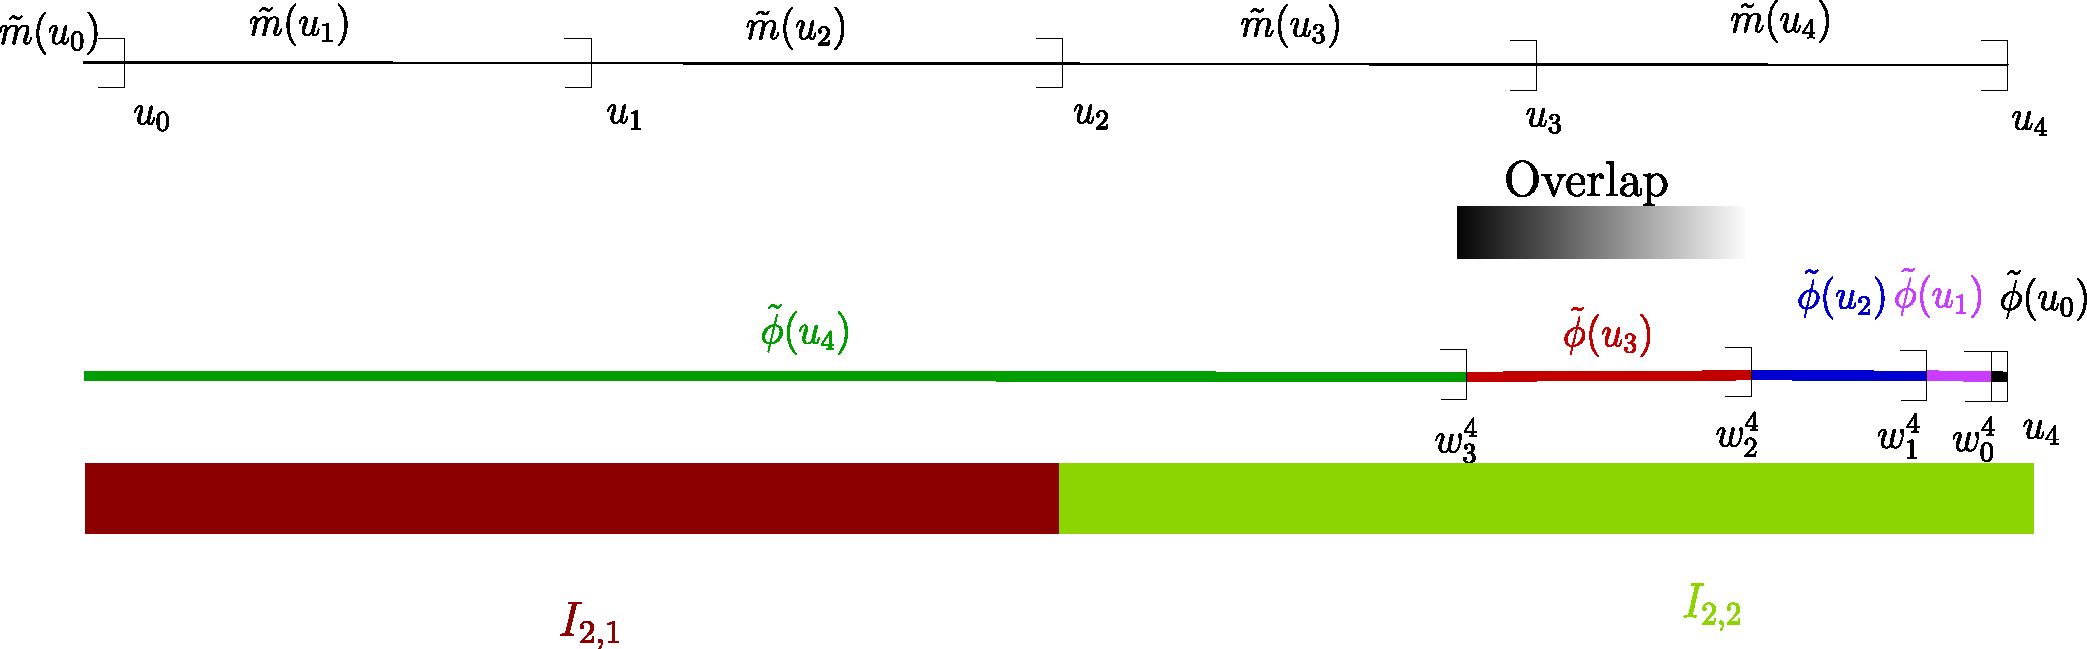
\includegraphics[width=\textwidth]{I2ls2}
        \caption{Visualization of discretization for $I_2$, where $n=3$}
        \label{fig:vis1}
    \end{figure}
\end{frame}
\begin{frame}
\frametitle{Transformation of the argument}
    Important to know: How many intervals do the $w$ spread? So find $n+1-j$ such that 
    \begin{equation*}
        w^{n+1}_i>u_j \quad\forall i=0\dotsc,n.
    \end{equation*}
    This can be calculated as
    \begin{equation*}
    l^*:=\left\lceil  \frac{u_n -w_{n}^{n+1}}{h}\right\rceil.
    \end{equation*}
    Is independent of $n$ because of the choice for $f$.
\end{frame}
\begin{frame}
    \frametitle{Transformation of the argument}
    What are the next steps?
    \begin{itemize}
        \item Divide $I_2$ into the different intervals
        \item the sorting of $(v_i)$ can be done it advance
        \item only shifting necessary in each timestep
    \end{itemize}
\end{frame}
\begin{frame}
    \frametitle{Transformation of the argument}
    \begin{table}
        \scriptsize
        \begin{tabular}{c|c|c|c|c}
            \# Elements & $\mathrm{L}^2$-error&EOC in $\mathrm{L}^2$&$\mathrm{L}^\infty$-error &EOC in $\mathrm{L}^\infty$\\
            \hline
            50 & 1.29927 & - & 0.0250247  & -\\
            100 & 0.450672 & 1.5275475676992607 & 0.0101168 & 1.3066064275748301\\
            200 & 0.153403 & 1.5547536813705434 & 0.00407696 &1.311182153107891\\
            400 & 0.0558441 & 1.4578457386762156 & 0.0017411 &1.2274971804453685\\
            800 & 0.0222726 & 1.3261379803853823 & 0.00147244  &0.2417923432251396
        \end{tabular}
        \caption{Convergence of the new algorithm for the simpler integral equation}
    \end{table}
\end{frame}
\begin{frame}
    \frametitle{Transformation of the argument}
    Everything works as it should. One might be tempted to think of effort $\mathcal{O}(N)$ but
    \begin{figure}
        \centering
        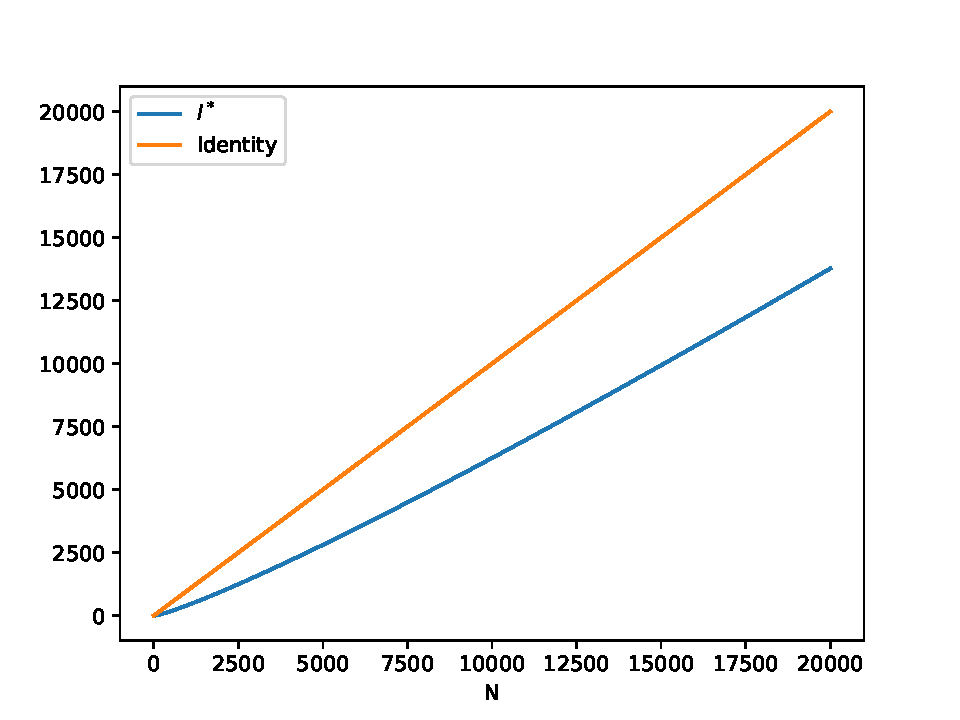
\includegraphics[width=0.5\textwidth]{runtime}
        \caption{Relationship of $l^*$ and $N$}
    \end{figure}
\end{frame}
\begin{frame}
    \frametitle{Transformation of the argument}
    Main takeaways:
    \begin{itemize}
       \item Unfortunately $\mathcal{O}(N^2)$ runtime
       \item but every timestep is equally fast
       \item good starting point for further studies
    \end{itemize}
\end{frame}
\section{Conclusion and outlook}
\begin{frame}
    \frametitle{Conclusion}
    \begin{itemize}[<+->]
        \item Simulation of a 2D problem 
        \item theoretical existence and uniqueness were proven
        \item results match physical expectations
        \item numerical convergence was obtained in practice
        \item simulation of a flow inside a rheometer cross section
        \item good starting for the integral without \enquote{\textsc{Laplace}} trick
    \end{itemize}
\end{frame}
\begin{frame}
    \frametitle{Outlook}
    Open questions:
    \begin{itemize}[<+->]
          \item Can the newly developed algorithm be altered to obtain runtime between $\mathcal{O}(N)$ and $\mathcal{O}(N^2)$?
          \item What if the flow is not only limited to one direction? 
          \item How can parallelization speed up the calculation? 
          \item How does one handle a continuous set of relaxation times?
          \item How can one use a simulation to perform parameter estimations?     
    \end{itemize}
\end{frame}
\begin{frame}
\huge{Thank you for your attention!}
\end{frame}
\end{document}
